
%
%  $Description: Author guidelines and sample document in LaTeX 2.09$ 
%
%  $Author: ienne $
%  $Date: 1995/09/15 15:20:59 $
%  $Revision: 1.4 $
%

\documentclass[times, 10pt,twocolumn]{article} 
\usepackage{latex8}
\usepackage{times}
\usepackage{epsfig}
\usepackage{graphicx}
\usepackage{subfigure}
\usepackage{amsmath}
\usepackage{amssymb}
\usepackage{color}
\usepackage{multirow}
\usepackage{url}
%\documentstyle[times,art10,twocolumn,latex8]{article}

%------------------------------------------------------------------------- 
% take the % away on next line to produce the final camera-ready version 
\pagestyle{empty}

%------------------------------------------------------------------------- 
\begin{document}

\title{Sketch/Image-Based 3D Scene Retrieval: Benchmark, Algorithm, Evaluation}

\author
       {
			  \begin{minipage}[b]{0.95\linewidth} % A minipage that covers half the page
        \centering
             Juefei Yuan$^{1}$, \hspace{1pt}	
						 Hameed Abdul-Rashid$^{1}$, \hspace{1pt}
							Bo Li$^{1}$\thanks{Corresponding author. For any questions, please contact Bo Li. E-mail: bo.li@usm.edu or li.bo.ntu0@gmail.com.}, \hspace{1pt}
							Yijuan Lu$^{2}$
       \end{minipage}
        \\
                 $^{1}$ School of Computing Sciences and Computer Engineering, University of Southern Mississippi, USA\\
                 $^{2}$ Department of Computer Science, Texas State University, San Marcos, USA\\								
				}
% ------------------------------------------------------------------------


\maketitle
\thispagestyle{empty}

\begin{abstract}
Sketch/Image-based 3D scene retrieval is to retrieve man-made 3D scene models given a user's hand-drawn 2D scene sketch or a 2D scene image usually captured by a camera. It is a brand new but also very challenging research topic in the field of 3D object retrieval due to the semantic gap in their representations: 3D scene models or views differ from either non-realistic 2D scene sketches or realistic 2D scene images.  Due to the intuitiveness in sketching and ubiquitous availability in image capturing, this research topic has vast applications such as 3D scene reconstruction, autonomous driving cars, 3D geometry video retrieval, and 3D AR/VR entertainment. To boost this interesting and important research, we build the currently largest and most comprehensive 2D scene sketch/image-based 3D scene retrieval benchmark\footnote
   {Our \textbf{Scene\_SBR\_IBR} benchmark: \url{http://orca.st.usm.edu/~bli/Scene_SBR_IBR/}.}, develop a convolutional neural network (CNN)-based 3D scene retrieval algorithm and finally conduct an evaluation on the benchmark. 

%The benchmark contains 750 scene sketches, 30000 scene images, and 3000 3D scene models, and all are equally classified into 30 classes. 

%We also conduct a thorough analysis and discussion on those methods, and suggest several future research directions to tackle this research problem. We wish this publicly available~\cite{SHREC18-SceneSBR-Track} benchmark, comparative evaluation results and corresponding evaluation code, will further enrich and advance the research of 2D scene sketch-based 3D scene retrieval and its applications.

%In this track, seven (7) groups from five countries (China, Chile, USA, UK, and Vietnam) have registered for the track, while due to many challenges involved, only three (3) groups have successfully submitted ten (10) runs of five methods. To have a comprehensive comparison, seven (7) commonly-used retrieval performance metrics have been used to evaluate their retrieval performance. We also suggest several future research directions for this research topic. We wish this publicly available~\cite{SHREC18-SceneIBR-Track} benchmark, comparative evaluation results and corresponding evaluation code, will further enrich and boost the research of 2D scene image-based 3D scene retrieval and its applications.


\end{abstract}

%------------------------------------------------------------------------- 
\Section{Introduction}
\label{sec:intro}
The huge and fast growing amount of 2D/3D scene files (sketches, images, and models) produced in our daily life makes researchers very excited since they shed bright light on many promising applications including autonomous driving cars,  3D scene reconstruction/retrieval, 3D geometry video retrieval, virtual reality (VR) and augmented reality (AR) in 3D entertainment, 3D game, animation and movie, 3D printing, and mobile applications. For instance,  2D sketch-based 3D scene retrieval and reconstruction facilitate the ability to create 3D scene contents for many 4D immersive programs, such as one of the most popular Disney World's programs -  Avatar Flight of Passage Ride~\cite{wiki:AvatarFlightofPassage, DisneyWorldAnimalKingdom, Pre-showinPandora}, and help us to find domain-specific indoor/outdoor 3D scenes, such as battlefield scenes for soldiers in training, sand table models for real estate marketing, or desert and mountain scenes for cartoon or game production. Therefore,  the benefits of this 3D scene retrieval research direction will be in its applications as well as across many related fields. 

%%%%%%%%%%%%%%%%%%%%%%%%%%%%%%%%%%%%%%%%%%%%%%%%
%%%%%%%%%%%%%%%%%%%%   SceneSBR    %%%%%%%%%%%%%%%%%%%%%%%%%%%%
%%%%%%%%%%%%%%%%%%%%%%%%%%%%%%%%%%%%%%%%%%%%%%%%
\textbf{Sketch-based 3D scene retrieval} is searching for relevant 3D scenes based on a 2D scene sketch input, which provides an intuitive and convenient scheme for users to learn and retrieve 3D scenes.  However, existing sketch-based 3D model retrieval algorithms~\cite{DBLP:journals/cviu/LiLLGSABCCFFFLLJKKOTWZZ15} have mainly focused on single object retrieval since they assume that there is only one object in a query sketch. Typically, there are several objects within a scene that may overlap one another, also occlusions are very common, and location configuration between objects provides helpful contextual information but is not trivial to interpret during retrieval. Nevertheless, considering its vast application scenarios, we believe that this research topic deserves further exploration and hopes to raise more interest and attention from people both inside and outside of the 3D object retrieval research community.


\textbf{Image-based 3D scene retrieval} finds relevant 3D scenes based on the content in a 2D scene query image, which also has vast related applications, including highly capable autonomous vehicles like the Renault SYMBIOZ \cite{Renault} \cite{Youtube}, multi-view 3D scene reconstruction, VR/AR scene content generation, and consumer electronics apps. 
However, similarly, there is a lack~\cite{xu2016data} of substantial research in this field due to the challenges involved and lack of related retrieval benchmarks. Seeing the benefits of advances in retrieving 3D scene models based on a scene image query makes this research direction useful, promising, and interesting as well. 

%It is also very promising and has great potentials in other related applications such as 3D geometry video retrieval, and highly capable autonomous vehicles like the Renault SYMBIOZ \cite{Renault} \cite{Youtube}. 


%due to the semantic gap existing between the iconic representation of 2D scene sketches and more accurate 3D representation of 3D scene models
%It is also very promising and has great potentials in many applications such as autonomous driving cars, 3D scene reconstruction, 3D geometry video retrieval, virtual reality (VR) and augmented reality (AR) in 3D Entertainment like Disney World's Avatar Flight of Passage Ride~\cite{wiki:AvatarFlightofPassage, DisneyWorldAnimalKingdom, Pre-showinPandora}.

%In addition, there are many existing 2D sketch-based 3D shape retrieval algorithms~\cite{DBLP:journals/cviu/LiLLGSABCCFFFLLJKKOTWZZ15} that usually targets the problem of retrieving a list of candidate 3D models using a single sketch as input, there is little existing research work on 2D scene sketch-based 3D scene retrieval. 

Although sketch/image-based 3D scene retrieval is an important and interesting research topic, it is extremely challenging due to the semantic gap in their representations: 3D scene models  differ from either non-realistic 2D scene sketches or realistic 2D scene images. Due to the wider representation gap between roughly outlined 2D scene sketches and precise 3D scene models, 2D scene sketch-based 3D scene retrieval (SceneSBR) is one of the most challenging research topics in 3D object retrieval. 

%%%%%%%%%%%%%%%%%%%%%%%%%%%%%%%%%%%%dataset%%%%%%%%%%%%%%%%%%
%\paragraph{Preliminary Work.} 
To promote this interesting yet challenging research, we organized two 2018 Eurographics Shape Retrieval Contest (SHREC) tracks~\cite{DBLP:conf/3dor/YuanLL18,  DBLP:conf/3dor/AbdulJLL18, SHREC18-SceneSBR-Track, SHREC18-SceneIBR-Track} titled ``2D Scene Sketch-Based 3D Scene Retrieval'' and ``2D Scene Image-Based 3D Scene Retrieval'',  by building the first 2D scene sketch/image-based 3D scene retrieval benchmark \textbf{SceneSBR} and \textbf{SceneIBR}. They share the same 1,000 3D scene models as the target dataset. \textbf{SceneSBR} contains 250 scene sketches, while \textbf{SceneIBR} has 10,000 2D scene images. All the sketches, images and models are equally classified into 10 indoor as well as outdoor classes. 

However, as can be seen, both benchmarks contain only 10 scene classes, and this is one of the reasons that all the three deep learning-based participating methods have achieved excellent performance. Considering this, after the track we have tripled the size of \textbf{SceneSBR} and \textbf{SceneIBR} to make each has 30 classes, and built an extended version for each, resulting a unified benchmark \textbf{Scene\_SBR\_IBR}, which has 750 2D scene sketches, 30,000 scene images, and 3,000 3D scene models. Similarly, all the 2D sketches, 2D images and 3D scenes are equally classified into 30 classes. 


%%%%%%%%%%%%%%%%%%%%%%%%%%%%%%%%%%%%%%%%%%%%%%%%
%%%%%%%%%%%%%%%%%%%%   algorithm and evaluation  %%%%%%%%%%%%%%%%%%%%%%%%%%%%
%%%%%%%%%%%%%%%%%%%%%%%%%%%%%%%%%%%%%%%%%%%%%%%%

In addition, to evaluate the new benchmark, we also propose a classification-based 3D scene retrieval algorithm based on the VGG~\cite{DBLP:journals/corr/SimonyanZ14a} deep learning model, considering the existing semantic gap in their representations. We develop our own 3D scene view sampling method; then simultaneously classify a query sketch/image and all the target 3D scenes via their scene views; and finally rank the 3D scenes accordingly to generate the retrieval algorithm's performance, which is provided as a baseline accuracy for the new benchmark. The main contributions introduced in this work are highlighted as follows:

%\paragraph{Problem $\&$ Significance.}
%\paragraph{Research Goal $\&$ Approach.}
%Therefore, now we can find that there is either a big \textbf{semantic gap} between 2D scene sketches and 3D scene models for 2D scene sketch-based 3D scene shape retrieval, or a scarce of substantial research in 2D scene image-based 3D scene shape retrieval due to its \textbf{challenges and difficulties}. 

%To our knowledge, CNN-SBR system performs best among all the existing retrieval systems that enable users to search 3D models based on hand-drawn 3D sketches. 

\begin{itemize}
    \item We propose a brand new research direction, that is sketch/image-based 3D scene retrieval, in the 3D Object Retrieval research area. 
    \item We build a new and the currently largest sketch/image-based 3D scene retrieval benchmark to promote this research direction. 		
    \item We evaluate the benchmark by using our newly proposed deep learning classification-based 3D scene retrieval algorithm and provide the baseline performance for the community. 
\end{itemize}


%First, we will further extend the 3D semantic tree to accommodate other types of shape data, such as 3D scene models, and 2D scene sketches/images. Then, we adapt the proposed semantic tree-based 3D scene retrieval framework for related applications research in the following areas: 1) semantics-driven 2D image-based 3D scene retrieval, 2) semantics-driven 2D scene sketch-based 3D scene retrieval, and 3) semantics-driven 2D scene sketch-based 3D scene reconstruction.

%The proposed novel semantic tree-based 3D scene retrieval framework will explicitly guide the research on sketch-based 3D scene retrieval and also provide a direction for sketch-based related applications and benefit many potential applications including virtual reality, gaming, 3D movie, and mobile apps. 


%\item \textcolor{red}{Educations? SHRECs?}


%\item



%------------------------------------------------------------------------- 
\Section{Related work}




%\textbf{3D scene datasets}:

%Lai:~\cite{DBLP:conf/icra/LaiBRF11, RGBDLAI}

%SUN3D:~\cite{DBLP:conf/iccv/XiaoOT13}

%100 scenes:~\cite{DBLP:journals/tog/FisherSH11}+~\cite{DBLP:journals/tog/XuCFSH13}

%\paragraph{Content-Based 3D Model Retrieval.} 3D models consist of 3D data (typically a list of vertices and faces) to represent 3D objects. 3D models are widely used in a lot of fields, such as industry product design, visualization and entertainment, 3D modeling, rendering, and animation. In recent years, the number of 3D models keeps increasing drastically, which triggers urgent research tasks and a lot of research interests in developing effective and efficient 3D shape retrieval algorithms for related applications. Given a query which is often a 2D sketch/image or a 3D model, content-based 3D model retrieval is to retrieve relevant 3D models (typically only single object models) coming from the same category as the query, and then rank them in the front part of the rank list as much as possible, while at the same time pushing irrelevant 3D models to the back of the rank list. Effectiveness, efficiency, and scalability are three most important performance metrics, which can be measured by a set of performance metrics commonly used in the field of information retrieval. 

%Most existing content-based 3D model retrieval algorithms target on single 3D object model retrieval, we are the \textbf{first} who built the first 3D scene retrieval benchmark~\cite{DBLP:conf/3dor/YuanLL18,  DBLP:conf/3dor/AbdulJLL18} based on either 2D scene image or sketch queries. We are also the first group who \textbf{pioneered} this research direction by organizing two  2018 Eurographics Shape Retrieval Contest (SHREC) tracks~\cite{SHREC18-SceneSBR-Track, SHREC18-SceneIBR-Track}.  

%\paragraph{2D Scene Sketch-Based 3D Scene Retrieval} 
%Sketching is a universal form of communication, which human have used to depict the visual world since prehistoric times. Today, sketching has become one of the most natural ways to search, such as retrieving images by sketching a scene on a smart phone and reconstructing a 3D scene model on the Internet by sketching the designed scene. Thus, we think sketch-based 3D scene retrieval has wider applications than sketch-based 3D model retrieval for single object models. 
%Currently, there is a lot of research in sketch-based 3D model retrieval~\cite{DBLP:journals/cviu/LiLLGSABCCFFFLLJKKOTWZZ15}. However, they usually target the problem of retrieving a list of candidate models using a single sketch as input. Therefore, the retrieval is ideally assumed as single sketch for single object, rather than in the context of a 2D scene sketch which contains several objects, which may overlap with each other and thus be occluded and also have relative location configurations. Therefore, sketch-based 3D model retrieval in the context of a 2D scene sketch query deserves our further explorations. 


\paragraph{3D scene retrieval.} Compared to sketch-based retrieval in the context of a single sketch, sketch-based retrieval using a 2D scene \textcolor{black}{sketch} query is much less studied. Fisher and Hanrahan \cite{DBLP:journals/tog/FisherHanrahan10} proposed a novel 3D model retrieval scheme named context-based 3D model retrieval, which is to retrieve models according to their spatial context in a 3D scene. They adopted a new pipeline of model retrieval by first locating the position of the model by drawing a 3D box and then searching relevant 3D models based on the dimensionality and context information. Models within scenes are extracted beforehand. Both geometry and tags are utilized to find related models based on the assumption that those models appear with similar contexts. However, our research topic differs from theirs in several facets. Firstly, their input is already a 3D scene consisting of several models. Secondly, the retrieval scheme is mainly for scene completion rather than scene reconstruction from scratch. Finally, they do not draw sketches to represent a 3D model or use an image as a template to build the scene. Recently, Xu et. al~\cite{DBLP:journals/tog/XuCFSH13} proposed Sketch2Scene for automatic 2D sketch-based 3D scene composition by representing 3D scene objects' functional and spatial relationships based on structural groups. 

%Sketch-based 3D model retrieval in the context of a 2D sketch of a scene, such as a 2D storyboard, is very important for the 3D scene reconstruction from a 2D sketch, as well. It is usually a fundamental step for 3D animation production guided by 2D storyboards \cite{Ta:2009:ODV:1578021.1578634}. This is mainly because sketches are more human-friendly and people are more accustomed to ``sketch'' their ideas using a set of sketches. In 3D animation production, 2D storyboards are often first drawn before reconstruction of the corresponding 3D scene. Proper 3D models are retrieved from available 3D databases to build a 3D scene \cite{Ta:2009:ODV:1578021.1578634} while keeping the context information in the original 2D scene consistent. 




%%%%%%%%%%%%%%%%%%%%%%%%%%%%%%%%%%%%%%%%%%%
\paragraph{2D/3D scene datasets.} %: techniques and benchmarks
Xiao et. al~\cite{DBLP:conf/cvpr/XiaoHEOT10} built the Scene UNerstanding (SUN) image database for the purpose of fostering improvements in  large scale scene recognition. SUN was initially comprised of 899 scene categories and 130,519 images. Later, SUN was extended to include 908 distinct classes \cite{DBLP:journals/ijcv/XiaoEHTO16}.  Xiao et. al~\cite{DBLP:conf/iccv/XiaoOT13} further created SUN3D, a RGB-D video database with camera pose and object labels, to capture full extend of 3D places. They used the videos for partial 3D reconstruction and propagated labels from one frame to another, then used the labels to refine the partial reconstruction. 
Song et. al~\cite{DBLP:conf/cvpr/SongYZCSF17} constructed SUNCG,  a database of synthetic 3D scenes with manually labeled voxel occupancy and semantic labels. SUNCG has 45,622 different scenes and 2,644 objects across 84 categories. 
Zhou et. al~\cite{DBLP:journals/pami/ZhouLKO018} compiled Places, a database of 10,624,928 scene images across 434 scene categories. While Places is not annotated at the object level, it provides the most diverse scene composition as well as insights into solutions to scene understanding problems. 

%\subsubsection{Zou et. al's SketchyScene dataset (2018)}
%Zou et. al~\cite{zou_eccv18} curated SketchyScene, a dataset with 29,000 scene-sketches, over 7,000 pairs of scene templates and photos, and  over 11,000 object sketches. Each scene is comprised of object-based semantic ground truths and instance mask. They also provided insights into the use of SketchyScene to explore potential methods trained to perform semantic segmentation as well as image retrieval, captioning and sketch coloring.




%Focal Points:~\cite{xu_sig14} scene object organizations analysis 




 % due to two major reasons 1) It is challenging to collect a large-scale 3D scene dataset and there exists a very limited number of available 3D scene shape benchmarks. 2) Like 2D sketch-based 3D shape retrieval, there is a big semantic gap between the iconic representation of 2D scene sketches and the accurate 3D coordinate representations of 3D scenes. All of above reasons make the task of retrieving 3D scene models using 2D scene sketch queries a challenging, although interesting and promising, research direction.

%Sketch-based 3D model retrieval has the intuitiveness advantage over other types of retrieval schemes. Currently, there is a lot of research in sketch-based 3D model retrieval, which usually targets the problem of retrieving a list of candidate 3D models using a single sketch as input. 

%\paragraph{2D Scene Image-Based 3D Scene Retrieval} 

%~\cite{xu2016data} 

%\Section{Our \textbf{Scene\_SBR\_IBR} benchmark\protect\footnote{Our \textbf{Scene\_SBR\_IBR} benchmark: \url{http://orca.st.usm.edu/~bli/Scene_SBR_IBR/Scene_SBR_IBR_Dataset.zip}}}
\Section{Our \textbf{Scene\_SBR\_IBR} benchmark}
\label{sec:benchmark}
\paragraph{Overview.} We have built a unified 3D scene benchmark supporting both sketch and model queries by substantially extending \textbf{SceneSBR} and \textbf{SceneIBR} by means of identifying and consolidating the same number of sketches/images/models for another additional 20 classes from the most popular 2D/3D data resources. Our work is the first to form a new and larger benchmark corpus for both sketch-based and image-based 3D scene retrieval. This benchmark provides an important resource for the community of 3D scene retrieval and will \textcolor{black}{likely} foster the development of practical sketch-based and image-based 3D scene retrieval applications.

\paragraph{Motivation.} 
As mentioned in Section~\ref{sec:intro}, to foster the research direction of sketch-based and image-based 3D scene retrieval, we built the first benchmark \textbf{SceneSBR} and \textbf{Scene\_IBR} respectively and organized two related Shape Retrieval Contest (SHREC) tracks~\cite{DBLP:conf/3dor/YuanLL18,  DBLP:conf/3dor/AbdulJLL18}. During the competitions, we found that both of these two benchmarks are not challenging and comprehensive enough since they cover only 10 categories, each of which is clearly distinct from one another. Considering this, we decided to further increase the comprehensiveness of the benchmarks by building a significantly larger and unified benchmark which supports both types of retrieval. 


%\paragraph{Preliminary Work.} 
%To promote this interesting yet challenging research, we organized two 2018 Eurographics Shape Retrieval Contest (SHREC) tracks~\cite{DBLP:conf/3dor/YuanLL18,  DBLP:conf/3dor/AbdulJLL18, SHREC18-SceneSBR-Track, SHREC18-SceneIBR-Track} titled ``2D Scene Sketch-Based 3D Scene Retrieval'' and ``2D Scene Image-Based 3D Scene Retrieval'',  by building the first 2D scene sketch/image-based 3D scene retrieval benchmark \textbf{SceneSBR} and \textbf{SceneIBR}. They share the same 1,000 3D scene models as the target dataset. \textbf{SceneSBR} contains 250 scene sketches, while \textbf{SceneIBR} has 10,000 2D scene images and all the sketches, images and models are equally classified into 10 classes. 

%However, as can be seen both benchmarks contain only 10 scene classes, which is one of the reasons that all the three deep learning-based participating methods have achieved excellent performance. Considering this, after the track we have tripled the size of \textbf{SceneSBR} and \textbf{SceneIBR} to make each has 30 classes, and built an extended version for each, resulting a unified benchmark \textbf{Scene\_SBR\_IBR}, which has 750 2D scene sketches, 30,000 scene images, and 3,000 3D scene models. Similarly, all the 2D sketches, 2D images and 3D scenes are equally classified into 30 classes. 

%The benchmark \textcolor{black}{was} motivated by the latest large collection of human-drawn sketches built by Eitz et al.~\cite{DBLP:journals/tog/EitzHA12}. 

\paragraph{Building process.} The first thing for the benchmark design is category selection, for which we have referred to several of the most popular 2D/3D scene datasets, such as Places~\cite{DBLP:journals/pami/ZhouLKO018} and SUN~\cite{DBLP:conf/cvpr/XiaoHEOT10}. Finally, we selected the most popular 30 scene classes (including the initial 10 classes in \textbf{SceneSBR} and \textbf{SceneIBR}) from the 88 available category labels in the Places88 dataset~\cite{DBLP:journals/pami/ZhouLKO018}, via a voting mechanism among three people (two graduate students as voters and a faculty member as the moderator) based on their judgments. We want to mention that the 88 common scenes are already shared by ImageNet~\cite{DBLP:conf/cvpr/DengDSLL009}, SUN~\cite{DBLP:conf/cvpr/XiaoHEOT10}, and Places~\cite{DBLP:journals/pami/ZhouLKO018}. Then, to collect data (sketches, images, and models) for the additional 20 classes, we gathered from Flicker and Google Image for sketches and images, and downloaded SketchUp 3D scene models (originally in .SKP format, but we provide .OBJ format as well after transformation) from 3D Warehouse~\cite{3DWareHouse}.


\paragraph{Benchmark details.} Our 3D scene retrieval benchmark \textbf{Scene\_SBR\_IBR} is publicly available\footnote{Available on the URL: \url{http://orca.st.usm.edu/~bli/Scene_SBR_IBR/}.}. All of its 30 classes has the same number of 2D scene sketches (25), 2D scene images (1000), and 3D scene models (100). It supports both sketch-based (via \textbf{Scene\_SBR}) and image-based (via \textbf{Scene\_IBR}) 3D scene retrieval by providing two different query datasets and a common 3D scene model target dataset:
\begin{itemize}
    \item \textbf{2D Scene Sketch Query Dataset (Subset 1).} The 2D scene sketch query set comprises 750 2D scene sketches (30 classes, each with 25 sketches). One example per class is demonstrated in \textbf{Fig.~\ref{BenchmarkSketchExamples}}.
    \item \textbf{2D Scene Image Query Dataset (Subset 2).} The 2D scene image query set is composed of 30,000 scene images (30 classes, each with 1,000 images). One example per class is demonstrated in \textbf{Fig.~\ref{BenchmarkImageExamples}}.
    \item \textbf{3D Scene Model Target Dataset (Subset 3).} The 3D scene dataset is built on the selected 3,000 3D scene models downloaded from Google 3D Warehouse. Each class has 100 3D scene models. One example per class is shown in \textbf{Fig.~\ref{BenchmarkSceneExamples}}.
\end{itemize}
Therefore, \textbf{Scene\_SBR\_IBR} is divided into two sub-level and task-specific benchmarks:  \textbf{Scene\_SBR} comprising \textbf{Subsets} 1 and 3 for sketch-based 3D scene retrieval and \textbf{Scene\_IBR} comprising \textbf{Subsets} 2 and 3 for image-based 3D scene retrieval. 


\begin{figure}[htb]
\centering
{
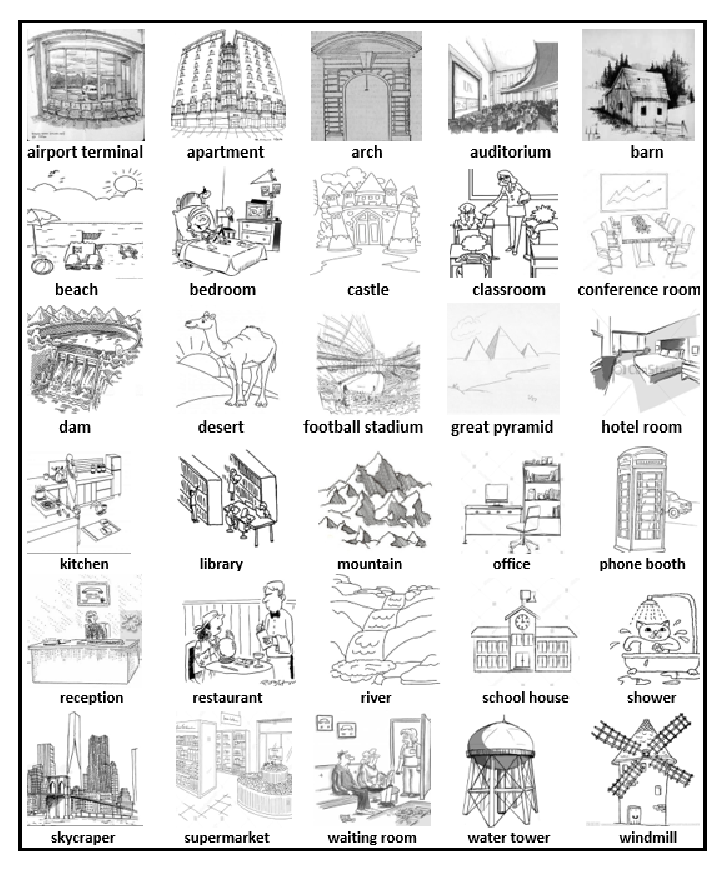
\includegraphics[width=1.0\linewidth]{SampleSketches}
}
\caption{Example 2D scene query sketches in our \textbf{Scene\_SBR\_IBR} benchmark. One example per class is shown.}
\label{BenchmarkSketchExamples}
\end{figure}


\begin{figure}[htb]
\centering
{
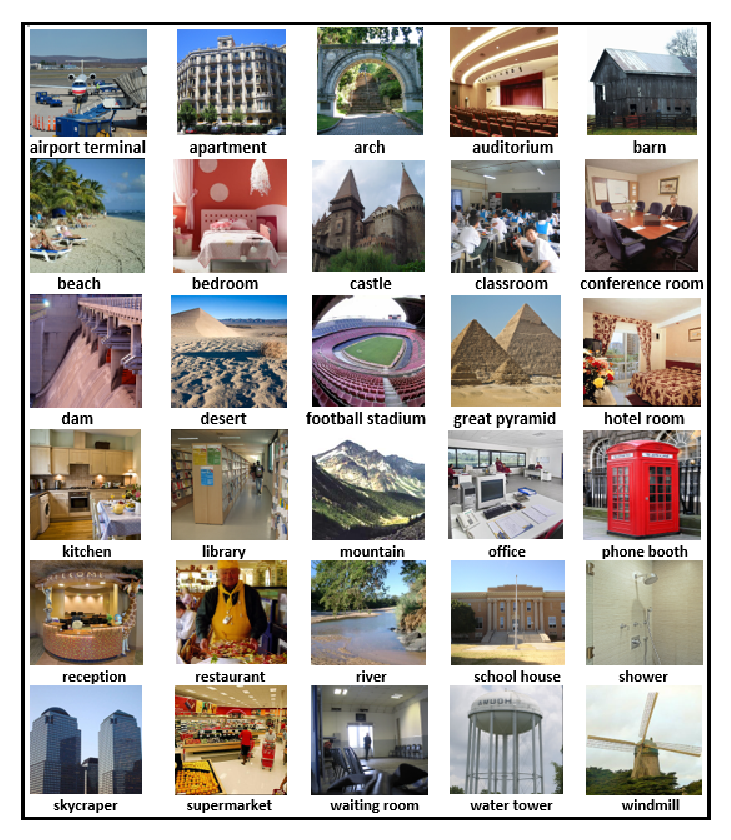
\includegraphics[width=1.0\linewidth]{SampleImages}
}
\caption{Example 2D scene query images in our \textbf{Scene\_SBR\_IBR} benchmark. One example per class is shown.}
\label{BenchmarkImageExamples}
\end{figure}


\begin{figure}[htb]
\centering
{
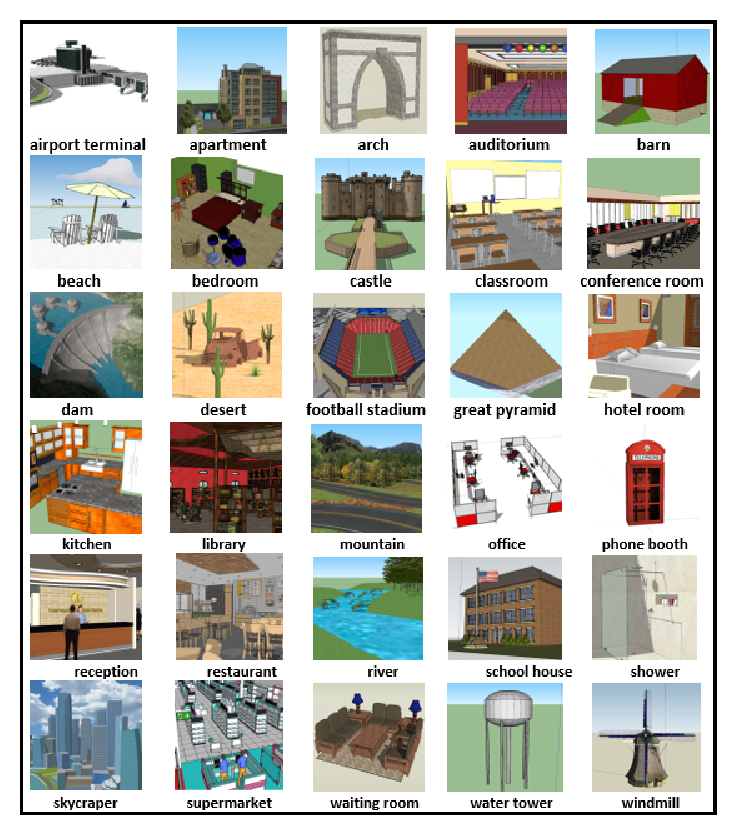
\includegraphics[width=1.0\linewidth]{SampleModels}
}
\caption{Example 3D target scenes in our \textbf{Scene\_SBR\_IBR} benchmark. One example per class is shown.}
\label{BenchmarkSceneExamples}
\end{figure}

To help evaluate learning-based 3D scene retrieval algorithms, we randomly select 18 sketches, 700 images, and 70 models from each class for training and use the remaining 7 sketches, 300 images, and 30 models for testing, as indicated in \textbf{Table}~\ref{table1}. The users are required to generate results based on the testing dataset if they use learning in their approach(es). Otherwise, the retrieval results can be generated based on the complete dataset.

\begin{table}[htb]
\centering
\caption {Training and testing dataset information of our \textbf{Scene\_SBR\_IBR} benchmark.}
\begin{center}
\begin{tabular}  {|c|c|c|c|}
 \hline
 \textbf{Datasets} & \textbf{Sketches} &\textbf{Images} & \textbf{Models} \\
 \hline
 \normalsize{Training (per class)}  & 18 &700  & 70  \\
 \hline
 \normalsize{Testing (per class)}  & 7 &300   & 30  \\
  \hline
 \normalsize{Total (per class)}  & 25 &1,000 & 100  \\
\hline
 \normalsize{Total (all 30 classes)}  &750 &30,000 & 3,000  \\
\hline
\end{tabular}
\end{center}
%\caption {Training and testing datasets (per class) of our \textbf{Scene\_SBR\_IBR} benchmark.}
\label{table1}
\end{table}

\paragraph{Evaluation metrics.}   
To have a comprehensive evaluation of a retrieval algorithm on our benchmark, we employ seven commonly adopted performance metrics in the 3D model retrieval community~\cite{DBLP:journals/cviu/LiLLGSABCCFFFLLJKKOTWZZ15}: Precision-Recall (PR) diagram, Nearest Neighbor (NN), First Tier (FT), Second Tier (ST), E-Measures (E), Discounted Cumulated Gain (DCG) and Average Precision (AP). We also have developed the related code to compute them for our benchmark.

%We target a real-time large-scale sketch/image-based 3D scene retrieval framework with good retrieval performance in terms of accuracy, efficiency and extensibility.  
%For the accuracy metrics, we employ seven commonly adopted performance metrics in the 3D model retrieval community~\cite{DBLP:journals/cviu/LiLLGSABCCFFFLLJKKOTWZZ15}: Precision-Recall (PR) diagram, Nearest Neighbor (NN), First Tier (FT), Second Tier (ST), E-Measures (E), Discounted Cumulated Gain (DCG) and Average Precision (AP). We will also develop the code to compute them. 
%Efficiency will be evaluated based on the average response time for a query, while extensibility will be assessed with respect to the framework's scalability to different scales of datasets, as well as diverse 2D/3D query/target formats, such as either 2D sketches or 2D images for queries, and 3D meshes, 3D point clouds, or RGB-D scans for the target dataset. 

\Section{Our retrieval algorithm \textbf{VMV-VGG}}
\label{sec:method}
%\paragraph{Architecture Overview.}~\label{sec:architecture} 
Based on the VGG-16 deep learning model~\cite{DBLP:journals/corr/SimonyanZ14a} and our prior work~\cite{DBLP:conf/icpr/Ye0L16}, we propose a View and Majority Vote based 3D scene retrieval algorithm (\textbf{VMV-VGG}), as illustrated in \textbf{Fig.}~\ref{architecture}. It employs two different VGG-16 based classification models (VGG1 and VGG2): one for 2D scene sketches/images, and the other for 2D scene views. For the model, we have the following parameter settings: the input image size: 256x256; the number of output categories: 30 for our proposed benchmark;  the batch size: 64; and the learning rate: 0.00001.

The retrieval algorithm comprises the following six steps: (1) {Scene view sampling:} we center each 3D scene model in a 3D sphere, and then automatically sample 13 scene view images based on a QMacro script program developed by us which automates the operations of the SketchUp software to perform the view sampling. For the 13 viewpoints, we uniformly sample 12 views along the equator of the sphere starting from the front view, and then sample one view from the north pole of the sphere. One example is demonstrated in \textbf{Fig.}~\ref{Sampleviewsexample}. 
(2) \textbf{Data augmentation:} to counter overfitting, before each pre-training or training, we first employ the same data augmentation technique we developed in~\cite{DBLP:conf/icpr/Ye0L16} to increase the related dataset's size by 500 times based on a set of random rotations, shifts and flips. 
(3)  \textbf{Pre-training of VGG1 and VGG2:} for sketch-based 3D scene retrieval we pre-train the VGG1 model on the TU-Berlin sketch dataset~\cite{DBLP:journals/tog/EitzHA12} at epoch 500, and pre-train VGG2 on the Places scene image dataset~\cite{DBLP:journals/pami/ZhouLKO018} at epoch 100; while for the image-based retrieval mode, we use Places to pre-train both VGG1 and VGG2 and stop at epoch 100. 
(4) \textbf{Fine-tuning:} fine-tune the pre-trained VGG1/VGG2 on the corresponding 2D scene sketches/images or 2D scene views training dataset at epoch 100/50, respectively. 
(5) \textbf{Sketch/image/view classification:} we respectively feed the well-trained model VGG1 or VGG2 with its corresponding testing query sketch/image or target scene view to obtain two classification vectors. 
(6) \textbf{Majority vote-based label matching:} finally we generate the rank list for each query by using majority vote-based label matching method based on the query's classification vector and a target 3D scene's 13 classification vectors.     

%For each 2D sketch/image query, we use VGG1 to classify which category each sketch/image belongs to based on the output similarity vector, which is for predicting categories. Each similarity vector contains 30 (the dataset has 30 categories) labels, the top first label that has the maximum similarity value in the similarity vector indicates the category of the query. Since we have 13 view based sampled images for each model, therefore, for each image, we had the second VGG-16 classification output similarity vector. 

%We use a majority vote algorithm to decide its final classification result based on the 13 output similarity vectors of its 13 2D images. Since the label of each sketch/image query was already classified first, therefore, for each testing scene model, the top first labels which match the sketch query label went to the top place of the retrieval result, the second top first which match the sketch query label was followed by the back, and so forth.  

\begin{figure}[htb]
\centering
{
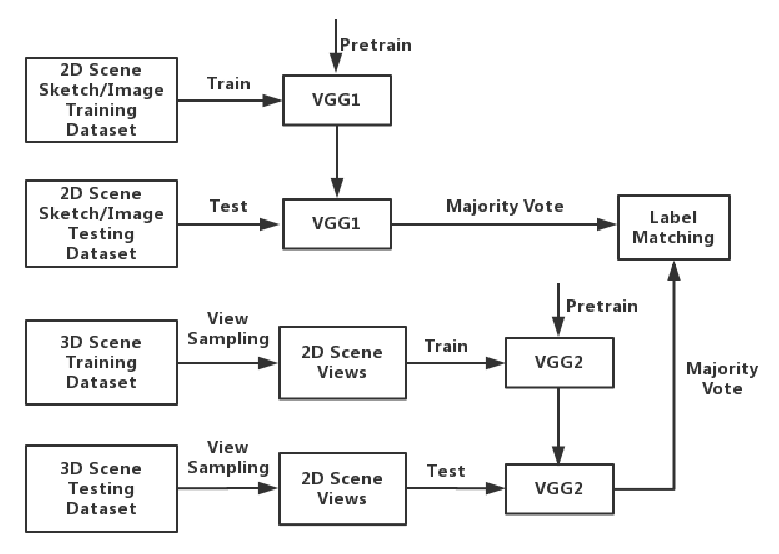
\includegraphics[width=1.0\linewidth]{architecture}
}
\caption{VBV-VGG architecture.}
\label{architecture}
\end{figure}


\begin{figure}[htb]
\centering
{
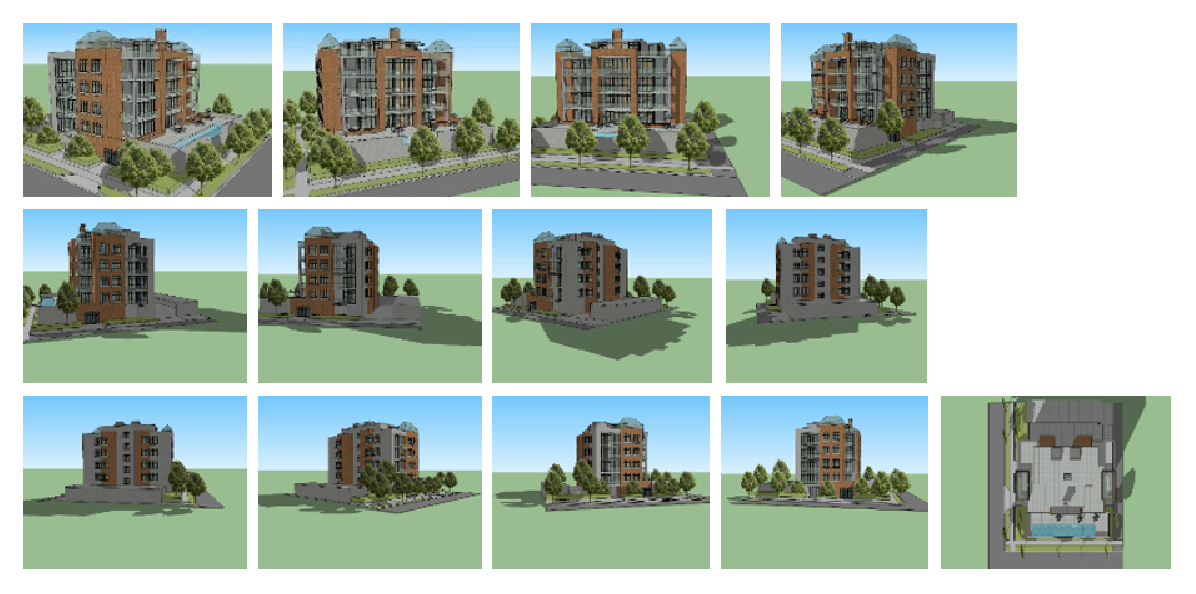
\includegraphics[width=1.0\linewidth]{Sampleviewsexample}
}
\caption{Scene view sampling example: a set of 13 sample views of an apartment scene model.}
\label{Sampleviewsexample}
\end{figure}

%\paragraph{Data augmentation}  for all the training data: to avoid overfitting, we also employ a data augmentation technique and expand the sizes of both the TU Berlin 2D sketch dataset and the obtained 2D sketch views from the training dataset by 500 times based on random rotations, shifts and flips. More specifically, we describe our data augmentation algorithm in Algorithm 1. By utilizing this algorithm, a sketch image will generate 500 new transformed images with one or more 2D image transformations of shift, rotation and flip. We introduce this random data augmentation algorithm to increase the variety of sketches, which significantly reduces the noises existing in users' hand-drawings.

%\paragraph{Scene view sampling.}~\label{sec:sample} 
 


\Section{Evaluation}
%\paragraph{Experiments}
%\label{sec:experiments}
The purpose of this evaluation is to provide the baseline performance for either sketch-based or image-based 3D scene retrieval on our benchmark \textbf{Scene\_SBR\_IBR} and also to examine the benchmark's comprehensiveness and difficulty level. To reach this purpose, we run our \textbf{VMV-VGG} algorithm presented in Section~\ref{sec:method} on the two sub-level benchmarks \textbf{Scene\_SBR} and \textbf{Scene\_IBR} of \textbf{Scene\_SBR\_IBR} respectively, by following the same parameter settings mentioned in Section~\ref{sec:method}. 

Their performance is shown in \textbf{Fig.}~\ref{fig:sbr18prperf} and \textbf{Table}~\ref{tab:SceneSBR} of \textbf{Scene\_SBR\_IBR} based on the seven performance evaluation metrics mentioned in Section~\ref{sec:benchmark}.  We have found that compared with the performance that has been achieved in the two SHREC'18 tracks~\cite{DBLP:conf/3dor/YuanLL18,  DBLP:conf/3dor/AbdulJLL18} which used a much smaller benchmark containing only 10 classes, in contrast to the current 30 classes available in our new benchmark, the overall performance dropped significantly for either type of retrieval. For example, Li's MMD-VGG method, which also utilizes VGG, has achieved an excellent overall performance in terms of DCG (0.856) or AP (0.685) on the \textbf{SceneSBR} benchmark, while they drop to DCG (0.533) and AP (0.244) respectively based on our \textbf{VMV-VGG}. This should be a direct and natural result after a substantial increase in the comprehensiveness and challenge level that exist in \textbf{Scene\_SBR\_IBR} after we incorporate much more scene categories. The addition of more classes will cause more ambiguities during the retrieval process and the retrieval algorithm may fail to properly distinguish between classes that share certain similarities. 

 %We plan to significantly extend the \textbf{Scene\_SBR\_IBR} benchmark by incorporating much more scene categories,

%To work on this, we propose that semantic information for detected objects in query images will help outline semantic attributes to be correlated with during the 3D scene retrieval process. The use of semantic object detection could potentially help with the inevitable ambiguities that exist between similar classes in a larger and more sophisticated dataset.

%The is mainly caused by the growth of the number of categories, it is more challenging for the deep neural network. More details about the retrieval performance of each individual query of every participating method can be found on the track homepage~\cite{SHREC18-SceneSBR-Track}.



%DCG performance fall from 0.864 to 0.533 for \textbf{Scene\_SBR}, and fall from 0.958 to 0.644 for \textbf{Scene\_IBR}.

%In addition, we can also find that 2D scene image-based 3D scene model retrieval has achieved much better performance than 2D scene sketch-based 3D scene model retrieval. We believe at least the following two main reasons contribute to the divergence. (1) \textbf{Scene\_IBR} has a much larger query dataset than \textbf{Scene\_SBR}, which should significantly contribute to obtaining a more powerful fine-tuned VGG1. (2) the query images in \textbf{Scene\_IBR} contain more details that the query sketches in \textbf{Scene\_SBR}. The additional color information in images can be used to correlate with the texture information existing in the 3D scene models (or their view images) during the retrieval. Therefore, the semantic gap between the query and testing datasets is much smaller than that of \textbf{Scene\_SBR}, making \textbf{Scene\_SBR} a much more challenging benchmark due to the huge semantic gap. 


%the 3D shape information is much more accurate than in \textbf{Scene\_SBR}'s query sketches; and (3) compared with the query sketches of \textbf{Scene\_SBR}, in each of \textbf{Scene\_IBR}'s query images, there are additional color information, which is correlated to the texture information in the 3D scene models. 




%\paragraph{Discussions}
%\label{sec:discussions}
%Though we cannot directly compare non-learning based approaches and learning-based approaches together, we have found much more promising results in learning-based approaches. The CNNs contribute a lot to the top performance of those four learning-based approaches for \textbf{Scene\_SBR} and \textbf{Scene\_IBR}. Considering many latest sketch/image based 3D model retrieval methods utilize deep learning techniques, we regard it as the currently most popular and promising machine learning technique for 2D/3D feature learning and related retrieval. In fact, the four methods that adopt certain deep learning models also perform well when adapted to this challenging benchmark.

%We classify all the participating methods with respect to the techniques employed: both of the two participating groups (Li, Yuan) utilize local features and both of them employ deep learning framework to automatically learn the features. But Li directly compute the 2D-3D distances based on the distributions of sketches/images and models by using the Euclidean distance metric, while Yuan conducts the retrieval based on 2D/3D classification.

%It can be seen from the corresponding figures and tables, for the same method each performance metric achieved on the \textbf{Scene\_IBR} is better than that on the \textbf{Scene\_SBR}. We believe at least the following three differences of \textbf{Scene\_IBR} contribute to its better performance: (1) it has a much larger query dataset which is very helpful for the training of the deep neural networks; (2) compared with the query sketches of \textbf{Scene\_SBR}, there is much more accurate 3D shape information in \textbf{Scene\_IBR}'s query images; and (3) each of \textbf{Scene\_IBR}'s query images has additional color information to correlate to the texture information existing in the 3D scene models. Therefore, there is a much smaller semantic gap to bridge between the query and target datasets for the \textbf{Scene\_IBR}, while the \textbf{Scene\_SBR} is much more challenging due to a big semantic gap there.


\begin{figure}[htb]
\centering
{
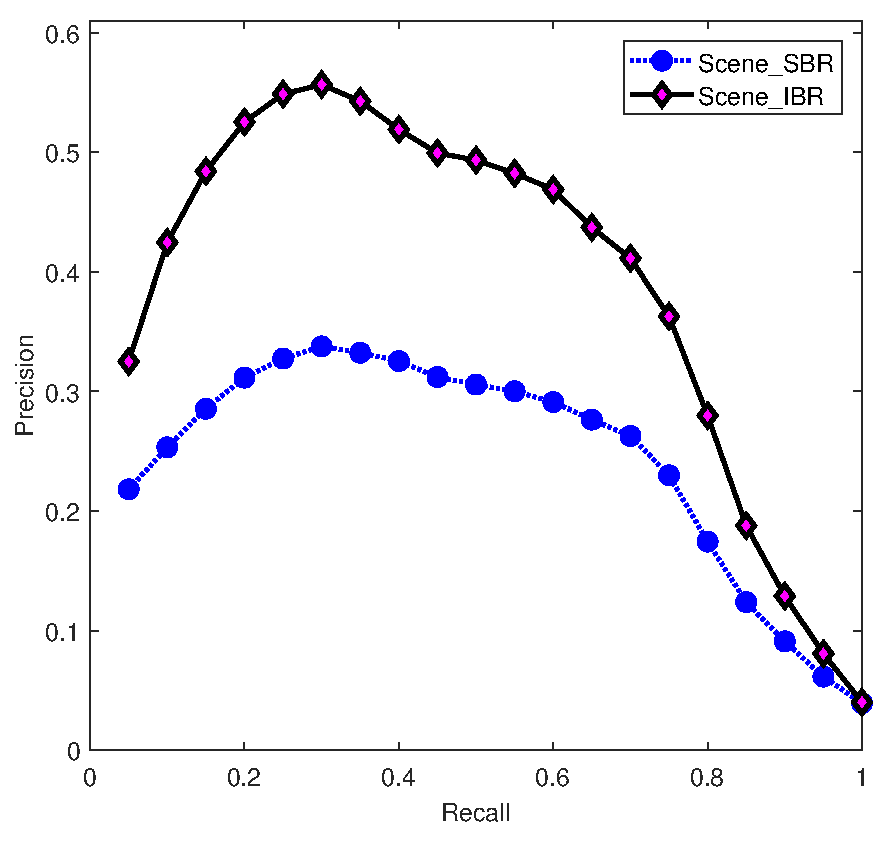
\includegraphics[height=0.82\linewidth]{comparative}
}
\caption{Precision-Recall diagram performance of our \textbf{VMV-VGG} on our \textbf{Scene\_SBR\_IBR} benchmark.}
\label{fig:sbr18prperf}
\end{figure}


\begin{table*}[htb]
	\centering
	\caption{Performance metrics generated by running our \textbf{VMV-VGG} on our \textbf{Scene\_SBR\_IBR} benchmark.}
	\label{tab:SceneSBR}
	\begin{tabular}{lccccccc}
			\hline		
	\normalsize {\textbf{Benchmark}} &\normalsize {\textbf{NN}}  &\normalsize {\textbf{FT}} &\normalsize {\textbf{ST}} &\normalsize {\textbf{E}} &\normalsize {\textbf{DCG}} &\normalsize {\textbf{AP}}\\
\hline
\textbf{Scene\_SBR}  &\textbf{0.081}	 &\textbf{0.281}	 &\textbf{0.369}	 &\textbf{0.280}	 &\textbf{0.533}  &\textbf{0.244}\\
\hline
\textbf{Scene\_IBR}  &\textbf{0.122}	 &\textbf{0.458}	 &\textbf{0.573}	 &\textbf{0.452}	 &\textbf{0.644}  &\textbf{0.392}\\				
\hline		
\end{tabular}
\end{table*}
%------------------------------------------------------------------------- 
\Section{Conclusions and future work}
Sketch/Image-based 3D scene retrieval are brand new, interesting, and challenging research topics with a lot of application potentials. There is extremely limited preliminary work in this field, which allows us to explore many promising ideas and interesting results. In this paper, the currently largest 3D scene retrieval benchmark \textbf{Scene\_SBR\_IBR} is proposed with the hope to advance this research direction. To assist other interested researchers, the baseline performance on the benchmark has been provided by conducting evaluation based on a proposed CNN classifier-based 3D scene retrieval algorithm \textbf{VMV-VGG}.  Our future goals include: (1) building a large-scale and/or multimodal 2D scene sketch/image-based 3D scene retrieval benchmark; (2) semantics-driven 2D scene sketch/image-based 3D scene retrieval.


%a further exploration of adaptively representing 3D sketches and 3D models using CNNs, and training our system for better 3D sketch and 3D model matching based on a larger collection of 3D sketches from more diverse users.

%This paper not only helps us identify state-of-the-art methods, but also existing problems, current challenges and future research directions for this important, new and interesting research topic.

%\textbf{(1) Large-Scale and/or Multimodal 2D Scene Sketch-Based 3D Scene Retrieval Benchmark.} Our proposed \textbf{\textbf{Scene\_SBR}} contains only 10 scene classes (even \textbf{Scene\_SBR\_IBR} only has 30 classes), which is one of the reasons that all the three deep learning-based participating methods have achieved excellent performance. For the next work, we plan to build a large-scale and/or multimodality 2D scene-based 3D scene retrieval benchmark considering that scalability to a large scale retrieval scenario and 2D/3D format diversities are very important for related applications. We plan to significantly extend the \textbf{Scene\_SBR\_IBR} benchmark by incorporating much more scene categories, as well as more modalities in either 2D queries (i.e. sketches and images) or 3D target models (i.e. RGD-D scenes, LIDAR scene images, and other scene range scans produced by other range scanners) format.  Then, we will arrange them on the scene semantic tree and organize another SHREC track on large-scale scene sketch-based 3D scene retrieval to invite people to adapt and run their algorithms on the new benchmark to evaluate their scalability in a large-scale and/or multimodal 3D scene retrieval scenario.


%\textbf{Semantics-driven 2D scene sketch/image-based 3D scene retrieval.} To improve either the accuracy or efficiency of a 2D scene sketch-based 3D scene retrieval algorithm, we need to consider utilizing the semantic information existing in both a 2D scene sketch query and all the 3D scene target models.  We believe related applications (i.e. online 3D scene retrieval, 3D Entertainment contents development, and autonomous driving cars) will benefit a lot from the retrieval based on extracted semantic information in both the queries and targets.

 %We plan to significantly extend the \textbf{Scene\_SBR\_IBR} benchmark by incorporating much more scene categories,

%The addition of more classes will cause ambiguity during the retrieval process and the model will fail to properly distinguish between classes that have similarities. To work on this, we propose that semantic information for detected objects in query images will help outline semantic attributes to be correlated with during the 3D scene retrieval process. The use of semantic object detection could potentially help with the inevitable ambiguities that exist between similar classes in a larger and more sophisticated dataset.



%\item \textbf{Semantics-driven 2D scene sketch-based 3D scene reconstruction.} The purpose is to reconstruct a 3D scene model guided by a 2D scene sketch as a design image by making the resulting 3D scene posses the same features as those in the design image. It involves 2D object detection and recognition, 3D model retrieval and pose alignment. It will be important for content generation for 3D Entertainment, VR/AR, 3D Animation and Movie applications. A deep learning-based object detection and semantic context information extraction module is utilized to facilitate retrieving the candidate models for the 3D reconstruction. The contextual and semantic information existing in the scene sketch could be utilized to select appropriate models and align the features of the models to the sketch features in the scene. %The framework of the initial idea is demonstrated in \textbf{Fig.}~\ref{reconstruction}  


%\item \textbf{Interdisciplinary research directions.} We have noticed the more outstanding performance achieved by Tran's 3D scene retrieval algorithm RNSRAP which is based on sketch and model classification. According to our previous class-based or semantic information-based 3D model retrieval research experience~\cite{DBLP:journals/mta/0013J13, DBLP:journals/mta/LiLJF17}, it is a promising approach to further improve retrieval accuracy, especially for NN, and FT since we can push more 3D scene models classified into one class forward to the front part of a retrieval rank list.

%-------------------------------------------------------------------------
\section*{Acknowledgments}
This project is supported by the University of Southern Mississippi Faculty Startup Funds Award to Dr. Bo Li and the Texas State Research Enhancement Program and  NSF CRI-1305302 Awards to Dr. Yijuan Lu. We gratefully acknowledge the support from NVIDIA Corporation for the donation of the Titan X/Xp GPUs used in this research. %, NSF CNS-1358939 and NSF OCI-1062439 Army Research Office grant W911NF-12-1-0057,
%------------------------------------------------------------------------- 
%\nocite{ex1,ex2}
\bibliographystyle{latex8}
\bibliography{latex8}

\end{document}

